\paragraph{$L^2$ minimisation (fixed $F_\text{obs}$).}
For any fixed observational CDF $F_\text{obs}$, the integral
$\int (F_\text{pred}(z) - F_\text{obs}(z))^2\,dz$
is non-negative and equals zero if and only if $F_\text{pred}(z) = F_\text{obs}(z)$ for all $z$. The minimiser over deterministic $F_\text{pred}$ is therefore $F_\text{obs}$ itself. This is an $L^2$ minimisation statement, not a propriety theorem in the \citet{gneiting2007strictly} sense---classical propriety requires an expectation over the random observation $y$, which the fixed-$F_\text{obs}$ statement does not involve.

\paragraph{Consistency under stochastic observations.}
Write $F_\text{obs}(y)$ for the observational CDF built from a specific draw $y$. The relevant quantity is
%
\begin{equation}
    \mathbb{E}_{y \sim Q} \bigl[ \text{CRPS}_\text{obs}(F_\text{pred}, F_\text{obs}(y)) \bigr].
\end{equation}
%
The metric should reward forecasts that get the location right, even when individual observations are noisy. Formally, I say that the pipeline is \emph{location-consistent} at $F_\text{pred} = Q$ if this expectation is minimised over the forecast location parameter when $F_\text{pred}$ equals the true data-generating distribution $Q$. Consistency in this sense is weaker than classical propriety---it depends on the $F_\text{obs}$ constructor being well-specified with respect to $Q$---but it is the property a practitioner needs: reporting the true location should yield the best expected score.

The honesty of the metric depends on the honesty of the $F_\text{obs}$ constructor. A practitioner who specifies $\sigma_\text{rel} = 0.3$ when the true relative uncertainty is 0.1 will get a metric that rewards forecasts that are too wide; one who specifies $\sigma_\text{rel}$ too small will get a metric that rewards overconfidence. The reformulation does not eliminate the distributional assumption---it moves it from inside the score formula to the constructor of $F_\text{obs}$, where it is visible, auditable, and open to sensitivity analysis.

\paragraph{Numerical consistency check.}
I verify consistency by drawing $N = 500$ observations $y^{(1)}, \ldots, y^{(N)}$ from a known log-normal truth with parameters $\mu_\text{true}$ and $\sigma = 0.3$ (a test parameter chosen for the numerical check; the operational default for conflict data is $\sigma_\text{rel} = 0.4$, \S3), constructing $F_\text{obs}(y^{(i)})$ parametrically for each draw with $\sigma_\text{rel} = 0.3$, sweeping a forecast parameter $\mu$ across a grid, and computing the expected score $\frac{1}{N}\sum_i \text{CRPS}_\text{obs}(F_\text{pred}(\mu), F_\text{obs}(y^{(i)}))$ for each $\mu$. The argmin should fall near $\mu_\text{true}$.

Figure~\ref{fig:propriety} shows the result for $\mu_\text{true} = 1.0$. At grid step $\Delta\mu = 0.05$ ($N = 500$ draws), the argmin falls on $\mu = 1.0$ for all four tested values $\mu_\text{true} \in \{0.5, 1.0, 1.5, 2.0\}$. Refining to $\Delta\mu = 0.005$ with $N = 2{,}000$ draws, the residual bias is $\leq 0.01$ and varies by seed---consistent with Monte Carlo noise at the grid resolution rather than a systematic shift.

\begin{figure}[h]
    \centering
    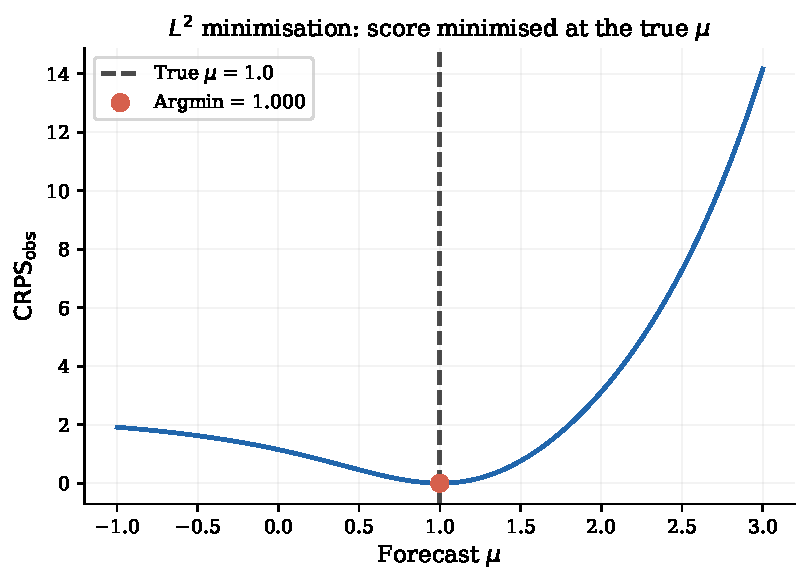
\includegraphics[width=0.65\textwidth]{figures/propriety_verification.pdf}
    \caption{Location-consistency check. The expected Cram\'er distance, averaged over $N = 500$ stochastic draws of $y$ from the true distribution (each with its own $F_\text{obs}(y^{(i)})$), is minimised at the true $\mu$.}
    \label{fig:propriety}
\end{figure}

\paragraph{Scale consistency: a convolution effect.}
The $\mu$-sweep above verifies location-consistency. A natural follow-up is whether the metric is also minimised at the true scale parameter $\sigma_\text{true}$. It is not---and the reason is intuitive: the metric rewards forecasts that match the truth \emph{as it would appear through the observation process}. Just as a blurred photograph combines camera-shake and lens-blur so that the result is wider than either source alone, the metric combines forecast spread and observation noise into a single effective width. For $\text{LogNormal}(\mu = 1.0, \sigma_\text{true} = 0.3)$ with observation-noise parameter $\sigma_\text{obs} = 0.3$ (equal to $\sigma_\text{rel}$ in the well-specified case), the expected Cram\'er distance is minimised at $\sigma_\text{pred} \approx 0.42$, not $0.30$. Under a Gaussian DGP ($\mu = 50$, $\sigma_\text{true} = 15$, $\sigma_\text{obs} = 10$), the argmin falls at $\sigma_\text{pred} \approx 18 \approx \sqrt{15^2 + 10^2}$. In both cases the minimiser is the convolution width $\sqrt{\sigma_\text{true}^2 + \sigma_\text{obs}^2}$: the expectation over stochastic $y$ effectively convolves $F_\text{pred}$ with the observation noise. For conflict fatality data, this effect is more consequential than in meteorology or hydrology: the RVI model of \citet{vesco2026uncertainty} implies observational uncertainty of $\sigma_\text{rel} \approx 0.2$--$0.9$ in log-space, which can equal or exceed forecast-model spread. When $\sigma_\text{obs} \geq \sigma_\text{true}$, the convolution width is dominated by observation noise, and the scale optimum shifts substantially from the true forecast spread.

The observable distribution is $Q * F_\varepsilon$, not the latent $Q$ itself. Classical CRPS has the same property in degenerate form: when $F_\text{obs} = \delta_y$ and $y = \theta + \varepsilon$, the CRPS-optimal forecast is $Q * F_\varepsilon$, not $Q$. Consistency therefore holds for location but not for scale: the metric rewards forecasts that match the observable data distribution, penalising overconfidence relative to what the data can actually resolve.
